\section{Theoretische Grundlagen}
    
    \subsection{Funktionsweise eines Lasers}
        Das Akronym Laser steht für 'light amplification by stimulated emission of radiation' und beschreibt eine Apparatur, die Licht einer bestimmten Wellenlänge aussendet, das über lange Strecken kohärent 
        ist und in Kombination mit der Möglichkeit besonders hoher Intensitäten und Pulsbarkeit sehr gut für experimentelle Anwendungen geeignet ist. Diese Eigenschaften werden ereicht, indem innerhalb eines 
        aktiven Mediums ein ausgewählter optischer Übergang angeregt und verstärkt wird. In diesem Versuch soll die Funktionsweise eines Laser kennengelernt und sich mit
        den Betriebsparametern eines Laser auseinandergesetzt werden. 
        
        \subsubsection{Anregungen und Übergänge im aktiven Medium}
            Um die grundlegende Funktionsweise eines Lasers zu verstehen müssen zunächst, die schematisch in Abbildung \ref{fig:prozesse} dargestellten, Absorptions- und Emissionsprozesse verstanden sein. Bei 
            der Absorption trifft ein Photon mit einer Energie, die der Energiedifferenz zwischen einem Zustand 1 und einem Zustand 2 entspricht, auf ein Atom und regt ein Elektron aus dem energetisch
            günstigeren Zustand 1 in den höhergelegenen Zustand 2 an. Bei der spontanen Emission relaxiert ein Elektron aus einem energetisch höheren Zustand 2 zufällig in einen niedriger gelegenen Zustand 2. Dabei 
            wird ein Photon ausgesendet, dessen Wellenlänge nach $\Delta E = E_2 - E_1 = \frac{\text{hc}}{\lambda}$ der Energiedifferenz der beteiligten Zustände entspricht. Richtung, Polarisation und Phase sind 
            zufällig gewählt. Bei dem 
            Prozess der stimulierten Emission trifft ein Photon auf ein angeregtes Atom. Wenn die Energie des einfallenden Photons der Energiedifferenz zwischen dem angeregten Zustand und einem energetisch
            niedrigeren Zustand entspricht, regt es das Elektron dazu an, aus dem angeregten Zustand in den energetisch günstigeren Zustand zurückzufallen. Dabei wird neben dem bereits vorhandenen Photon ein
            weiteres emittiert, das kohärent zu dem Einfallenden ist. Das heißt, dass Frequenz, Wellenvektor, Phase und Polarisation der beiden Photonen identisch sind.      


            \begin{figure}[h]
                \centering
                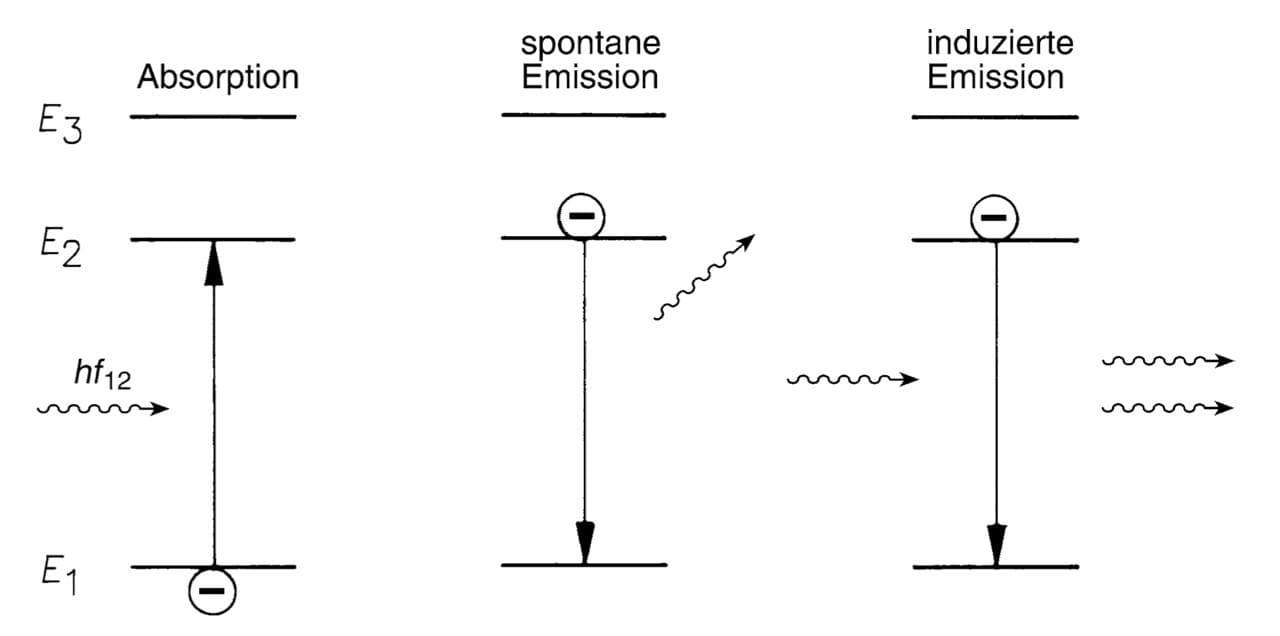
\includegraphics[width = 0.7\textwidth]{pictures/prozesse.jpg}
                \caption{Die Prozesse der Absorption, spontanen sowie induzierten Emission sind schematisch dargestellt. $E_{1,2,3}$ bezeichnen verschiedene atomare Energieniveaus, $h$ das Planck`sche Wirkungsquantum und $f_{1,2}$ die Frequenz des Photons, die propotional zur Energiedifferenz zwischen den Energien 1 und 2 ist. Entnommen aus \cite{eichler_laser_2015}.}
                \label{fig:prozesse}
            \end{figure}
            
            \FloatBarrier


            Bei einem HeNe-Laser findet der optische Übergang innerhalb der Neon-Atome statt. Dazu müssen diese zunächst in einen angeregten Zustand bewegt werden. Dies geschieht über eine Energiepumpe, die 
            in diesem Fall über Gasentladungen verwirklicht wird. Bei diesen wird im Laserrohr, das das HeNe-Gemisch beinhaltet eine Spannung angelegt, die bei Entladung Helium-Atome anregt. Die angeregten 
            He-Atome stoßen mit den Ne-Atomen und übertragen dabei ihre Energie, sodass die He-Atome wieder im Grundzustand und die Ne-Atome nun angeregt sind. Im Falle eines roten Laser mit einer Wellenlänge 
            von \SI{632.9}{\nano\metre} muss das Ne-Atom nun aus dem angeregten Zustand in einen energetisch günstigeren Zustand übergehen, sodass die Energiedifferenz zwischen den Zuständen einem Photon
            der gegebenen Wellenlänge entspricht. Wie in Abbildung \ref{fig:termschema} zu sehen, entspricht dies einem Übergang aus dem $3s_2$- in den $2p_4$-Zustand.

            \begin{figure}[h]
                \centering
                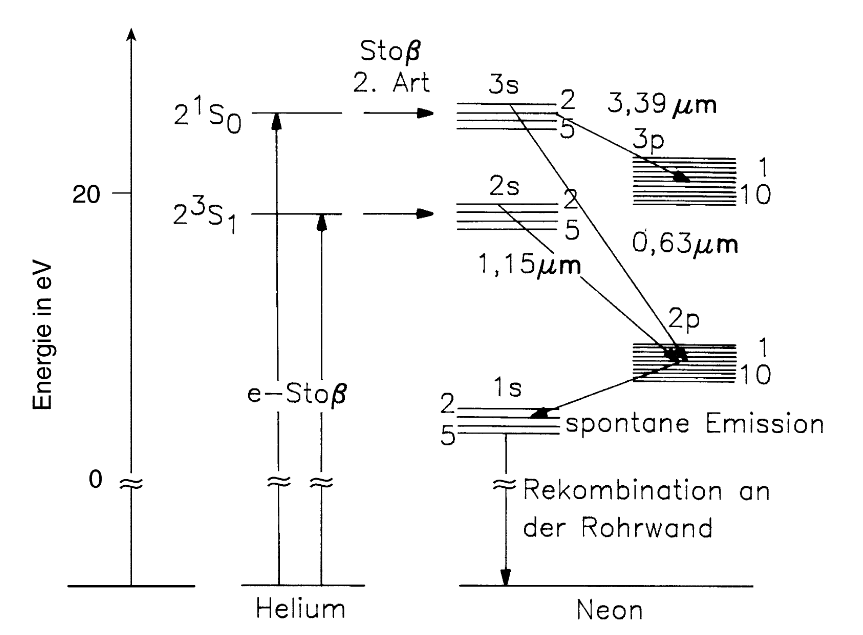
\includegraphics[width = 0.7\textwidth]{pictures/Termschema.png}
                \caption{Das Schema der beteiligten Energieniveaus innerhalb eines HeNe-Lasers zeigt die zunächst durch Gasentladungen angeregten He-Zustände und die involvierten Zustände innerhalb des Ne-Atoms. Entnommen aus \cite{eichler_laser_2015}.}
                \label{fig:termschema}
            \end{figure}

            \FloatBarrier
            

        \subsubsection{Besetzungsinversion}
            Um einen solchen Übergang dauerhaft zu ermöglichen muss eine Besetzungsinversion der beiden Zustände erreicht werden. Dies bedeutet, dass der energetisch höhere Zustand mit der Besetzungszahl $N_2$ 
            stärker besetzt ist als der energetisch günstigere Zustand mit der Besetzungszahl $N_1$ ($N_2 > N_1$). In einem System aus zwei Energieniveaus ist dies unmöglich und auch in einem System aus drei 
            Niveaus ist es sehr schwer, da der energetisch günstige Zustand der Grundzustand ist und demnach sehr stark gepumpt werden muss, um eine Besetzungsinversion zu erreichen. Daher sind wie in Abbildung 
            \ref{fig:termschema} zu sehen, meist mehr als drei Niveaus beteiligt. Zur Beschreibung der Besetzungsinversion wird die Ratengleichung genutzt. Diese beschreibt die Änderung der Besetzung eines 
            bestimmten Zustands mit der Zeit. Dazu werden zum einen die Prozesse betrachtet, die zum Verlust von Elektronen aus diesem Zustand führen. Dazu gehören spontane und induzierte Emission. Zum anderen werden 
            die Prozesse betrachtet, die zum Anstieg der Elektronenzahl in diesem Zustand führen. Dazu wiederum gehören Emissionsprozesse aus höheren Energieniveaus oder Absorptionsprozesse in niedrigeren 
            Energieniveaus, bei denen Elektronen in den betrachteten Zustand angeregt werden. Im stationären Betrieb ist die Änderung der Differenz der am optischen Übergang beteiligten Zustände konstant und 
            der Laser emittiert stabil Licht.      


        \subsubsection{Selektive Verstärkung eines Übergangs}
            Zur selektiven Verstärkung des gewünschten optischen Übergangs wird ein optischer Resonator genutzt, der stimulierte Emission zwischen den gewünschten Energieniveaus ermöglicht, indem er spontan
            emittierte Photonen der gewünschten Wellenlänge mehrfach durch das Laserrohr laufen lässt. Daher besteht der Resonator aus zwei Spiegeln, die das Laserlicht reflektieren. Damit der Resonator stabil 
            ist, muss die Feldverteilung des Laserstrahls nach jedem Durchlauf durch das Laserrohr wieder gleich sein. Dies ist gegeben, wenn die Stabilitätbedingung
            
            \begin{equation*}
                0 < g_1g_2 < 1 \qquad \text{oder} \qquad g_1=g_2=0 \qquad \text{mit} \qquad g_{\text{i}} = 1 - \frac{d}{b_{\text{i}}},
                \label{eqn:Stabilitätsbedingung}
            \end{equation*}

            die von der Resonatorlänge $d$ und den verwendeten Spiegelradien $b_{\text{i}}$ abhängt, erfüllt ist. In Abbildung \ref{fig:stabilität} sind die Verläufe der Stabilitätbedingung zugehörigen Kurven 
            für die verwendeten Spiegelkombinationen dargestellt. Für die zwei konkaven Spiegel mit einem Krümmungsradius von jeweils \SI{1.4}{\metre} ergibt sich eine maximale Resonatorlänge von 
            \SI{2.8}{\metre}, die der Summe der Krümmungsradien entspricht. Für die Kombination eines planaren Spiegels mit einem konkaven Spiegel des Krümmungsradius \SI{1.4}{\metre} entspricht die maximale 
            Resonatorlänge dem Krümmungsradius des konkaven Spiegels und damit \SI{1.4}{\metre}.
            
            \FloatBarrier
            %%%%%%%%%%%%%%%%%%%%%%%%%%%%%%%%%%% Hier den Stabilitätsgraphen einfügen %%%%%%%%%%%%%%%%%%%%%%%% 
            \begin{figure}[h]
                \centering
                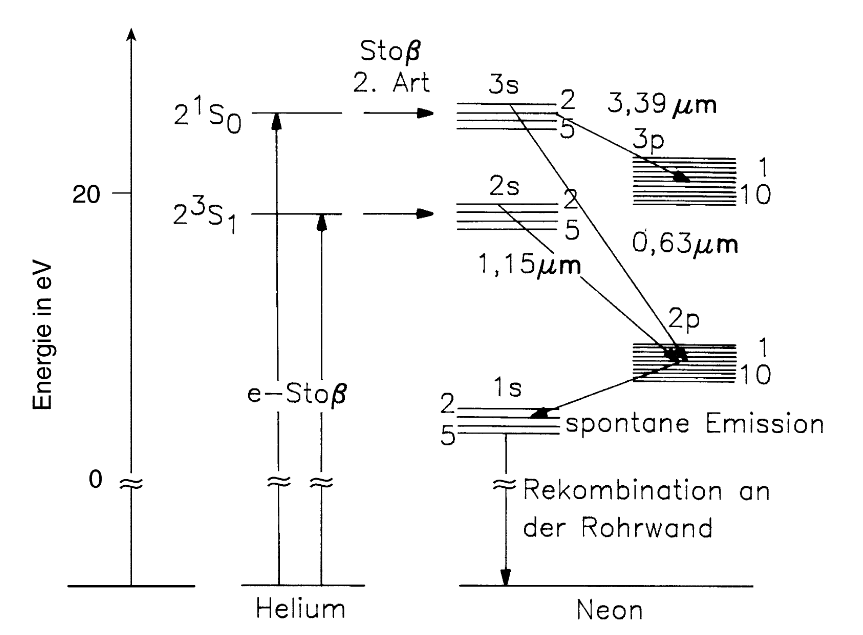
\includegraphics[width = 0.7\textwidth]{pictures/Termschema.png}
                \caption{Eine grafische Abbildung der Stabilitätbedingung, aus der erkennbar ist, dass die maximale Resonatorlänge bei einer Kombination zweier identischer konkaven Spiegeln dme doppelten Krümmunsgradius entspricht. Für die Kombination eines planaren Spiegels mit einem konkaven Spiegel entspricht die maximale Resonatorlänge dem Krümmungsradius des konkaven Spiegels.}
                \label{fig:stabilität}
            \end{figure}

            \FloatBarrier


            Bei erfüllter Stabilitätbedingung durchlaufen die Photonen nun mehrfach das Laserrohr und können bei erreichter Besetzungsinversion wiederholt stimulierte Emission hervorrufen. Diese exponentielle 
            Vervielfachung der Photonen soll zur Verstärkung der Lichtintensität führen, die ab einer erfüllten Schwellwertbedingung eintritt. Dazu wird zunächst die Verstärkung G definiert

            \begin{equation}
                \text{G} = \left(\frac{I}{I_0}\right) = \exp \left[-2\left(N_{\text{i}} - \frac{g_{\text{i}}}{g_{\text{k}}}N_{\text{k}}\right)\sigma(f)\text{L} - \gamma\right],
                \label{eqn:Verstärkung}
            \end{equation}

            die das Verhältnis zwischen Ausgangsleistung $I_O$ und Endleistung $I$ nach einem Durchlauf durch den Resonator angibt und von der Besetzung des energetisch höheren Zustands $N_{\text{k}}$, der des 
            energetisch niedrigeren Zustands $N_{\text{i}}$, deren statistischen Gewichtungen $g_{\text{i,k}}$, dem frequenzabhängigen Absorptionquerschnitt des Übergangs von Zustand k zu Zustand i $\sigma (f)$
            der Resonatorlänge L und dem Faktor $\gamma$, der die Reflektions- und Streuverluste pro Durchlauf zusammenfasst, abhängt. Die Lichtintensität wird erhöht (G>1), wenn die Schwellwertbedingung

            \begin{equation*}
                N_{\text{i}} - \frac{g_{\text{i}}}{g_{\text{k}}}N_{\text{k}} > \frac{\gamma}{2\sigma (f) L}
                \label{eqn:Schwellwertbedingung}
            \end{equation*}

            erfüllt ist, also die Verstärkung durch hohe Besetzungsinversion stark genug ist, um die Verluste pro Durchlauf zu übersteigen. Nun werden immer mehr kohärente Photonen der gewünschten Wellenlänge 
            erzeugt und so dieser spezielle Übergang verstärkt.


        \subsubsection{Modenausbildung innerhalb des Resonators}
            Während des stationären Betriebs des Laser bilden sich innerhalb des Resonators spezielle Moden des elektrischen Feldes aus. Diese werden in transversale und longitudinale Moden unterteilt. 
            Transversale Moden bilden sich senkrecht zum Wellenvektor des elektrischen Feldes und longitudinale Moden parallel zu diesem aus. Die Struktur dieser Moden lässt sich berechnen, indem die 
            Wellengleichung des elektrischen Feldes innerhalb des Resonators gelöst wird. \newline
            Die transversalen Moden ergeben sich dabei aus den Lösungen der Wellengleichungen im achsennahen Bereich entlang der Ausbreitungsrichtung, die einer Gaußglocke multipliziert mit einem 
            Hermite-Polynom pro transversaler Achse $H_{\text{n,m}}$ entsprechen:

            \begin{equation*}
                E(x,y) = E_0 H_{\text{n}}(x) H_{\text{m}}(y) \exp \left(-\frac{x^2+y^2}{w_0^2}\right) \qquad \text{mit} \qquad H_{\text{n}}(x) = (-1)^{\text{n}} \text{e}^{x^2} \frac{\text{d}^{\text{n}}}{\text{d}x^{\text{n}}} e^{-x^2} 
            \end{equation*}

            Dabei beschreibt $w_0$ den minimalen Radius des Strahls.
            In diesem Versuch sollen im speziellen die transversalen elektrischen Moden TEM$_{00}$ und TEM$_{10}$ entlang der x-Achse vermessen werden, deren Feldverteilungen entlang der x-Achse in Abbildung 
            dargestellt sind. Unter der Annahme einer Messung entlang der x-Achse ($y=0$) ergeben sich nach $I \propto E^2$ folgende Intensitätsverteilungen für die beiden Moden: 
            

            \begin{align}
                \text{TEM}_{00}:& \qquad I(x) = I_0 \exp \left(-\frac{2x^2}{w_0^2}\right) \\
                \text{TEM}_{10}:& \qquad I(x) = I_0 \frac{8x^2}{w_0^2} \exp \left(-\frac{2x^2}{w_0^2}\right)
            \end{align}
                
            Demnach entspricht die messbare Intensitätsverteilung der TEM$_{00}$-Mode einer Gauglocke. Die Intensitätsverteilung der TEM$_{10}$-Mode entspricht einer Gauglocke multipliziert mit einer 
            Parabel.\newline

            \begin{figure}[h]
                \centering
                \includegraphics[width = 0.7\textwidth]{pictures/Intensität.jpg}
                \caption{Die Feldverläufe der TEM$_{00}$- und TEM$_{10}$-Mode sind entlang der x-Achse aufgetragen. Entnommen aus \cite{demtroder_laserspektroskopie_2011}.}
                \label{fig:Intensität}
            \end{figure}

         

            Die Lösung der Wellengleichung in longitudinaler Richtung ergibt eine Vielzahl an Moden, die gleichzeitig entstehen können, sofern ihre Frequenz in dem Bereich liegt, der nach \ref{eqn:Verstärkung}
            eine Verstärkung der Lichtintensität erlaubt. Die Moden sind dabei alle um die Frequenz $\Delta f$ 

            \begin{equation*}
                \Delta f = \frac{\text{c}}{2\text{d}},
            \end{equation*}

            die sich aus der Resonatorlänge d und der Lichtgeschwindigkeit c ergibt, voneinander entfernt. Um einen Laser mit einer einzelnen longitudinalen Mode zu betreiben kann ein Etalon in den 
            Strahlengang eingesetzt werden. Dabei handelt es sich um einen weiteren Resonator, dessen Spiegelabstand deutlich kleiner ist als der des Laseresonators. Dies führt dazu, dass der Modenabstand 
            hier viel größer ist. Nun bleiben nur die longitudinalen Moden erhalten, die mit einer Etalonmode übereinstimmen und die anderen werden unterdrückt. Aufgrund des größeren Modenabstands kann so eine
            einzelne longitudinale Mode im Intensitätverstärkenden Bereich ausgewählt werden. 

        \subsubsection{Polarisation des Laserstrahls}
            Um den Laser mit einer vorgeschriebenen Polarisation zu betreiben, werden an den Enden des Laserrohrs Brewster-Fenster installiert. Diese transmittieren den zur Einfallsebene parallel polarisierten
            Anteil zu 100\% und den senkrecht polarisierten Anteil nur zu circa 60\%. Dies führt dazu, dass nur die Verluste für den parallel polarisierten gering genug sind, um eine Intensitätverstärkung zu 
            erreichen und so diese Polarisationsrichtung als einzige erhalten bleibt, da Photonen aus stimulierter Emission ebenfalls diese Polarisartion tragen werden.  


    \subsection{Interferenz am Gitter}
        Wenn teilkohärentes Licht auf ein Gitter trifft kommt es zu Interferenz. Dies liegt daran, dass sich nach dem Huygen´schen an den Gitterlinien Elementarwellen ausbilden, die untereinander interferieren.
        Dabei kommt es zu konstruktiver Interferenz, wenn der Gangunterschied, also die Distanz die eine Elementarwellen zurücklegt, bevor die nächste ausgesendet wird, einem ganzzahligen Vielfachen der 
        Wellenlänge entspricht:

        \begin{equation}
            \Delta s = k \lambda \qquad \text{mit} \qquad k \in \mathds{Z}
            \label{eqn:gangunterschied}
        \end{equation}

        \begin{figure}[h]
            \centering
            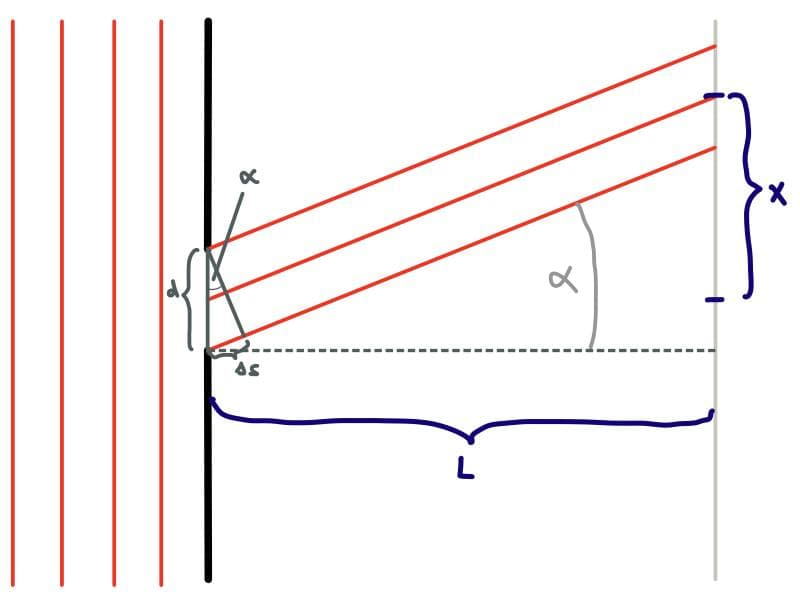
\includegraphics[width = 0.7\textwidth]{pictures/spalt.jpg}
            \caption{Skizze aller relevanten geometrischen Parameter bei der Beugung an einem Einzelspalt.}
            \label{fig:Spalt}
        \end{figure}

        Über die in Abbildung \ref{fig:Spalt} zu sehende geometrische Betrachtung des Interferenzbildes für einen Einzelspalt lassen sich für Interferenzmaxima folgende Beziehungen erkennen

        \begin{align*}
            \sin \left(\alpha\right) &= \frac{\Delta s}{d} \\
            \sin \left(\alpha\right) &= \frac{x_k}{\text{L}} ,
        \end{align*}

        die den Ablenkwinkel $\alpha$ mit dem Gangunterschied $\Delta s$, dem Abstand zwischen Gitter und Schirm L und der Gitterkonstante $d$ und dem Abstand vom Maximum nullter Ordnung zum Maximum k-ter 
        Ordnung $x_k$ verknüpfen und auch für ein Gitter gelten. In Kombination mit der Bedingung für den Gangunterschied \ref{eqn:gangunterschied} lässt sich so eine Formel zur Bestimmung der Wellenlänge aufstellen

        \begin{equation}
            \lambda = \frac{d}{k} \sin\left[\arctan \left(\frac{x_k}{L}\right) \right],
            \label{eqn:Wellenlänge}
        \end{equation}

        die für jedes Maximum valide ist.